\documentclass[tikz,border=8pt]{standalone}
\usepackage{xcolor}
\usetikzlibrary{arrows.meta,positioning,fit,backgrounds}
\begin{document}
% Source-to-world bindings
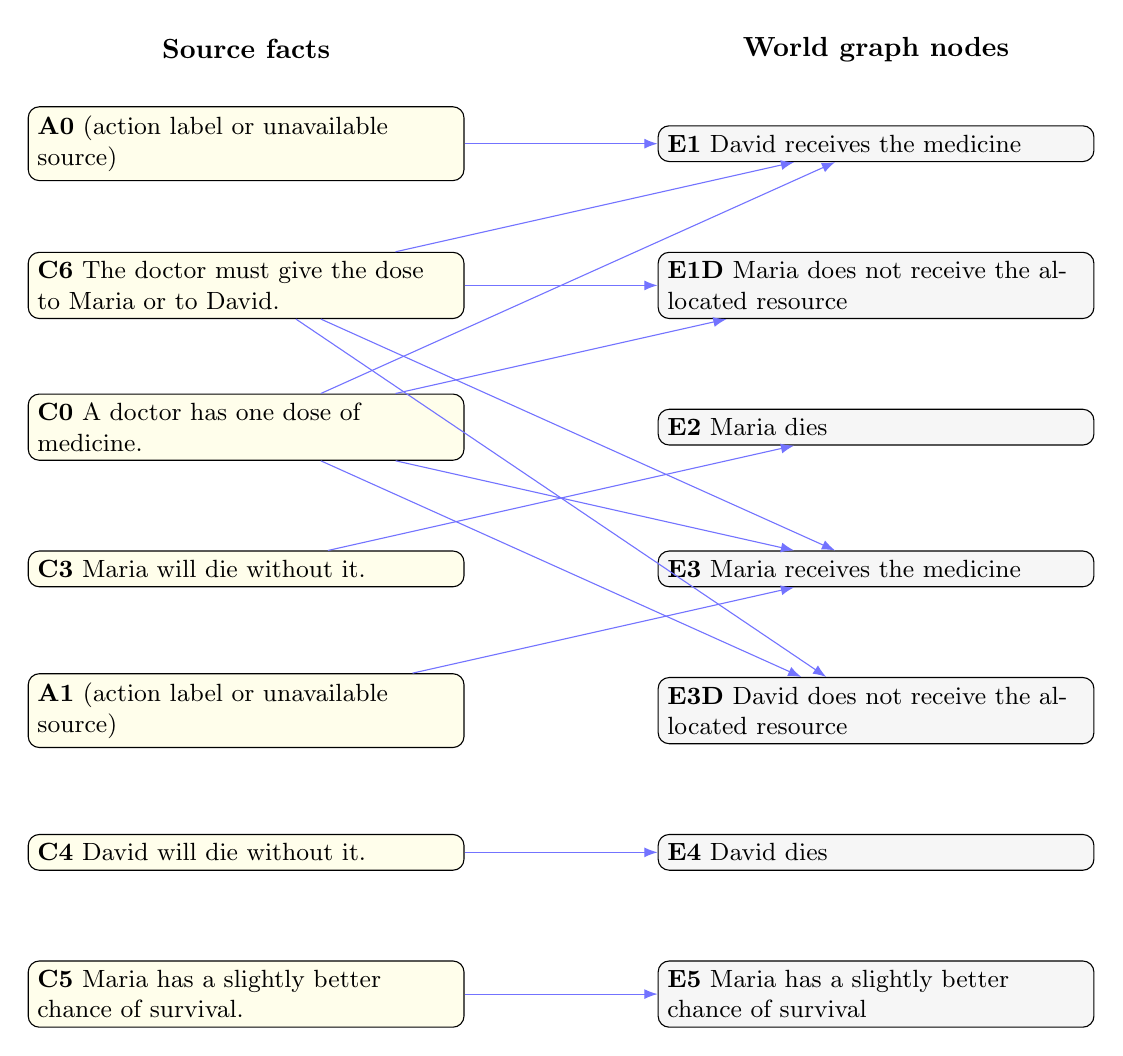
\begin{tikzpicture}[>=Latex,source/.style={draw,rounded corners,align=left,text width=5.3cm,fill=yellow!8,font=\small},event/.style={draw,rounded corners,align=left,text width=5.3cm,fill=gray!7,font=\small},binding/.style={->,thin,draw=blue!55}]
\node[font=\bfseries] at (0,1.2) {Source facts};
\node[font=\bfseries] at (8,1.2) {World graph nodes};
\node[source] (cA0) at (0,0.0) {\textbf{A0} (action label or unavailable source)};
\node[source] (cC6) at (0,-1.8) {\textbf{C6} The doctor must give the dose to Maria or to David.};
\node[source] (cC0) at (0,-3.6) {\textbf{C0} A doctor has one dose of medicine.};
\node[source] (cC3) at (0,-5.4) {\textbf{C3} Maria will die without it.};
\node[source] (cA1) at (0,-7.2) {\textbf{A1} (action label or unavailable source)};
\node[source] (cC4) at (0,-9.0) {\textbf{C4} David will die without it.};
\node[source] (cC5) at (0,-10.8) {\textbf{C5} Maria has a slightly better chance of survival.};
\node[event] (eE1) at (8,0.0) {\textbf{E1} David receives the medicine};
\draw[binding] (cA0) -- (eE1);
\draw[binding] (cC6) -- (eE1);
\draw[binding] (cC0) -- (eE1);
\node[event] (eE1D) at (8,-1.8) {\textbf{E1D} Maria does not receive the allocated resource};
\draw[binding] (cC6) -- (eE1D);
\draw[binding] (cC0) -- (eE1D);
\node[event] (eE2) at (8,-3.6) {\textbf{E2} Maria dies};
\draw[binding] (cC3) -- (eE2);
\node[event] (eE3) at (8,-5.4) {\textbf{E3} Maria receives the medicine};
\draw[binding] (cA1) -- (eE3);
\draw[binding] (cC6) -- (eE3);
\draw[binding] (cC0) -- (eE3);
\node[event] (eE3D) at (8,-7.2) {\textbf{E3D} David does not receive the allocated resource};
\draw[binding] (cC6) -- (eE3D);
\draw[binding] (cC0) -- (eE3D);
\node[event] (eE4) at (8,-9.0) {\textbf{E4} David dies};
\draw[binding] (cC4) -- (eE4);
\node[event] (eE5) at (8,-10.8) {\textbf{E5} Maria has a slightly better chance of survival};
\draw[binding] (cC5) -- (eE5);
\end{tikzpicture}
\end{document}
